	\documentclass[10pt,oneside]{CBFT_book}
	% Algunos paquetes
	\usepackage{amssymb}
	\usepackage{amsmath}
	\usepackage{graphicx}
	\usepackage{libertine}
	\usepackage[bold-style=TeX]{unicode-math}
	\usepackage{lipsum}

	\usepackage{natbib}
	\setcitestyle{square}

	\usepackage{polyglossia}
	\setdefaultlanguage{spanish}
	



	\usepackage{CBFT.estilo} % Cargo la hoja de estilo

	% Tipografías
	% \setromanfont[Mapping=tex-text]{Linux Libertine O}
	% \setsansfont[Mapping=tex-text]{DejaVu Sans}
	% \setmonofont[Mapping=tex-text]{DejaVu Sans Mono}

	%===================================================================
	%	DOCUMENTO PROPIAMENTE DICHO
	%===================================================================

\begin{document}

% =================================================================================================
\chapter{Conceptos fundamentales de electromagnetismo}
% =================================================================================================


% =================================================================================================
\section{Ecuaciones de Maxwell}
% =================================================================================================

Son ecuaciones lineales de modo que vale la superposición (con \vb{E}, \vb{B} y 
cualquier vector relacionado linealmente con ellos).
\[
	\nabla \cdot \vb{D} = 4 \pi \rho_\ell \qquad \nabla \cdot \vb{B} = 0
\]
\[
	\nabla \times \vb{E} = - \frac{1}{c} \dpar{B}{t} \qquad \nabla \times \vb{H} =
	\frac{4\pi}{c} \vb{J}_\ell + \frac{1}{c}\dpar{D}{t}
\]
\[
	\vb{F} = q \left( \vb{E} + \frac{1}{c} \vb{v} \times \vb{B} \right)
\]

Los vectores pueden ser polares (tienen físicamente bien definido el sentido) o
axiales (se les atribuye un sentido por convención).

Las ecuaciones son invariantes ante transformaciones del tipo: rotación
y reflexión espacial y temporal.

% =================================================================================================
\section{Electrostática}
% =================================================================================================

La ley de Coulomb reza que
\[
	\vb{F}_{12} = q_1 q_2 \frac{(\vb{x}_1 - \vb{x}_2)}{|\vb{x}_1 - \vb{x}_2 |^3}
\]
que es la fuerza sobre 1 debido a 2. De la ley de Coulomb se puede definir 
\[
	\vb{E}_{12}(\vb{x}_1) \equiv \vb{F}_{12}/q_1
\]
y tomando $\vb{x}_1 \equiv \vb{x}$ y haciendo el límite $q_1 \to 0$ se tiene
\[
	\vb{E}(\vb{x}) = \sum_{i=1}^N \; q_i \frac{(\vb{x} - \vb{x}_i)}{|\vb{x} - \vb{x}_i |^3}
\]
que es el campo eléctrico y que en el paso al continuo resulta
\[
	\vb{E}(\vb{x}) = \int_{V'} \rho(\vb{x}) \frac{(\vb{x} - \vb{x}_i)}{|\vb{x} - \vb{x}_i |^3} dV' 
\]
siendo \vb{x} punto campo y $\vb{x}_i$ punto fuente.

\begin{figure}[htb]
	\begin{center}
	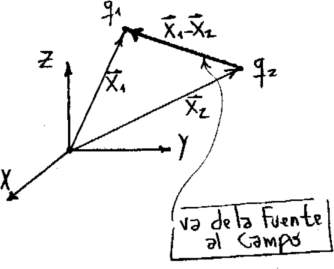
\includegraphics[width=0.6\textwidth]{images/fig_ft1_ejescargas.pdf}	 
	\end{center}
	\caption{}
\end{figure} 

\subsection{Conservación de la carga}

La carga total sale de una integral 
\[
	Q = \int_{V'}  \rho(\vb{x}') dV'
\]
como muestra la imagen
\begin{figure}[htb]
	\begin{center}
	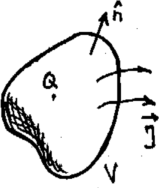
\includegraphics[width=0.25\textwidth]{images/fig_ft1_conserv.pdf}	 
	\end{center}
	\caption{}
\end{figure} 
y si el volumen es fijo podemos tomar la derivada con respecto al tiempo que pasa el interior como
derivada parcial,
\[
	\dtot{Q}{t} = \int_{V'} \dpar{\rho}{t} (\vb{x}') dV' = - \int_{S\equiv\partial V'} \vb{J} \cdot d\vb{S}
\]
y el miembro extremo derecho  se debe a que si la carga varía es a consecuencia de que se va en
forma de flujo. Aplicando el teorema de la divergencia en el miembro derecho,
\[
	\int_{V'} \dpar{\rho}{t} (\vb{x}') dV' = - \int_{V'} \nabla \cdot \vb{J} \; dV'
\]
lo cual vale para todo volumen y entonces esto significa que
\[
	\dpar{\rho}{t} + \nabla \cdot \vb{J} = 0
\]
que es la ecuación de continuidad de la carga. Si fuera $\nabla \cdot \vb{J}=0$ esto significa que las líneas
de \vb{J} no tienen principio ni fin.

% =================================================================================================
\section{Interacción magnética}
% =================================================================================================

Cuando se da $\nabla \cdot \vb{J}=0$ hablamos de una corriente estacionaria (no hay acumulación de carga en
ninguna parte). Las corrientes estacionarias producen efectos magnéticos dados por la ley de Biot-Savart
\[
	\vb{B}(\vb{x}) = \frac{1}{c} \int_\Gamma \frac{I d\vb{\ell}' \times (\vb{x} - \vb{x}')}{|\vb{x} - \vb{x}'|^3} 
\]
que es válida para un circuito $\Gamma$, que es una curva que se recorre en sentido CCW.
En el caso de un volumen la expresión es 
\[
	\vb{B}(\vb{x}) = \frac{1}{c} \int_{V'} \frac{ \vb{J}(\vb{x}') \times (\vb{x} - \vb{x}')}{|\vb{x} - \vb{x}'|^3} 
dV'
\]
mientras que la fuerza sobre un circuito $\Gamma$ es
\[
	F = \frac{1}{c} \int_\Gamma I d\vb{\ell} \times \vb{B}
\]
y sobre un volumen 
\[
	F = \frac{1}{c} \int_V \vb{J} \times \vb{B} dV
\]

La transformación entre estas integrales puede hacerse merced al siguiente razonamiento,
% \begin{align*}
%  	I d\vb{\ell} \times \vb{B} = \vb{J}  \cdot d\vb{S} d\vb{\ell}  \times \vb{B} =
%   	\cos(\theta) dS \vb{J} d\ell \times \vb{B} = \\
% 	\vb{J} \times \vb{B}  \cos(\theta) dS d\ell  = \vb{J} \times \vb{B}  d\vb{S} \cdot d\vb{\ell}  = 
% 	\vb{J} \times \vb{B}  dV 
% \end{align*}
\[
  	I d\vb{\ell} \times \vb{B} = \vb{J}  \cdot d\vb{S} d\vb{\ell}  \times \vb{B} =
  	\cos(\theta) dS \vb{J} d\ell \times \vb{B} = 
\]
\[
	\vb{J} \times \vb{B}  \cos(\theta) dS d\ell  = \vb{J} \times \vb{B}  d\vb{S} \cdot d\vb{\ell}  = 
	\vb{J} \times \vb{B}  dV 
\]

\subsection{Fuerza de un circuito sobre otro}

La fuerza de un circuito 2 sobre otro circuito 1 puede calcularse con un poco de paciencia como sigue
\[
	F_{12} = \frac{1}{c} \int_{\Gamma_1} I_1 d\vb{\ell}_1 \times \left\{
	\frac{1}{c} \int_{\Gamma_2} \frac{I_2 d\vb{\ell}_2 \times (\vb{x}_1 - \vb{x}_2)}{|\vb{x}_1 - \vb{x}_2|^3} 
	\right\}
\]
\[
	F_{12} = \frac{I_1 I_2}{c^2} \int_{\Gamma_1} \int_{\Gamma_2} d\vb{\ell}_1 \times \left\{
	\frac{d\vb{\ell}_2 \times (\vb{x}_1 - \vb{x}_2)}{|\vb{x}_1 - \vb{x}_2|^3} 
	\right\}
\]
\[
	F_{12} = \frac{I_1 I_2}{c^2} \int_{\Gamma_1} \int_{\Gamma_2} d\vb{\ell}_2  \left\{
	\frac{d\vb{\ell}_1 \cdot (\vb{x}_1 - \vb{x}_2)}{|\vb{x}_1 - \vb{x}_2|^3} 
	\right\} - \int_{\Gamma_1} \int_{\Gamma_2} \frac{ (\vb{x}_1 - \vb{x}_2)}{|\vb{x}_1 - \vb{x}_2|^3} 
	\left\{ d\vb{\ell}_1 \cdot d\vb{\ell}_2 \right\}
\]
donde el primer término se comprueba nulo si se reescribe utilizando que
\[
	\frac{ (\vb{x}_1 - \vb{x}_2)}{|\vb{x}_1 - \vb{x}_2|^3} = 
	\nabla_{\vb{x}_2} \frac{ 1 }{|\vb{x}_1 - \vb{x}_2|} =
	- \nabla_{\vb{x}_1} \frac{ 1 }{|\vb{x}_1 - \vb{x}_2|} 
\]
de manera que entonces
\[
	- \int_{\Gamma_2} d\vb{\ell}_2  \int_{\Gamma_1} d\vb{\ell}_1 \cdot \nabla_{\vb{x}_1} \frac{ 1 }{|\vb{x}_1 - \vb{x}_2|} 
\]
donde se ve que es nula la última integral dado que 
\[
	\int_{\Gamma_1} d\vb{\ell}_1 \cdot \nabla_{\vb{x}_1} = 0.
\]

Entonces, se tiene 
\[
	F_{12} = - \frac{I_1 I_2}{c^2} \int_{\Gamma_1} \int_{\Gamma_2} \frac{ (\vb{x}_1 - \vb{x}_2)}{|\vb{x}_1 - \vb{x}_2|^3} 
	\left( d\vb{\ell}_1 \cdot d\vb{\ell}_2 \right)
\]
que vale lo mismo si intercambiamos $\Gamma_1$ con $\Gamma_2$ en la integración. Podemos decir que con corrientes estacionarias
vale el principio de acción y reacción: las fuerzas son iguales y de sentido opuesto.


% =================================================================================================
\section{Teorema de Helmholtz}
% =================================================================================================

Nos dice que un campo vectorial está completamente determinado por su divergencia y su rotor.
Por ejemplo, para un campo eléctrico 
\[
	\vb{E} = \int_{V'} \rho \frac{\vb{x} - \vb{x}'}{|\vb{x} - \vb{x}'|^3} dV' = 
		- \int_{V'} \rho \nabla_{\vb{x}} \frac{ 1 }{|\vb{x} - \vb{x}'|} dV' = 
		- \nabla_{\vb{x}} \int_{V'}   \frac{ \rho }{|\vb{x} - \vb{x}'|} dV' = 
\]
y esta última es la integral de Poisson
\[
	\vb{E} = - \nabla_{\vb{x}} \phi (\vb{x}).
\]
Entonces $\vb{E}$ es un gradiente y por ello 
\[
	\nabla  \times \vb{E} = 0
\]
de manera que $\vb{E}$ es conservativo, cumple $\int \vb{E}\cdot d\vb{\ell} = 0$ o lo que
es lo mismo, $\vb{E}$ es irrotacional.
Hemos hecho la construcción de un potencial electrostático.

% =================================================================================================
\section{Ley de Gauss}
% =================================================================================================



\begin{figure}[htb]
	\begin{center}
	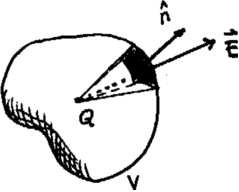
\includegraphics[width=0.35\textwidth]{images/fig_ft1_gauss.pdf}	 
	\end{center}
	\caption{}
\end{figure} 
\[
	\vb{E} \cdot \hat{n} = q \frac{\cos(\theta)}{r^2}
\]
y el ángulo sólido es
\[
	\vb{E} \cdot \hat{n} dS = q \frac{\cos(\theta)}{r^2} dS
\]
\[
	\vb{E} \cdot \hat{n} dS = q d\Omega \qquad \longrightarrow \qquad 
	\int_{S\equiv\partial V} \vb{E} \cdot \hat{n} \; dS = q \int_S d\Omega =
	\begin{cases}
	 0 \quad \textrm{carga exterior}\\
	 4\pi \quad \textrm{carga interior}
	\end{cases}
\]
\[
	\int_S \vb{E} \cdot \hat{n} \; dS = 4\pi \sum_i q_i
\]
La ley de Gauss es
\[
	\int_S \vb{E} \cdot \hat{n} \; dS = 4\pi Q_n
\]
donde $Q_n$ es la carga neta dentro de la superficie $S$. Al continuo pasa como 
\[
	\int_S \vb{E} \cdot \hat{n} \; dS = 4\pi \int_V \rho \: dV
\]
de manera que 
\[
	\int_V \divem{E} \; dV = \int_V 4\pi \rho \: dV
\]
y entonces
\[
	\divem{E} = 4\pi \rho.
\]

Por otro lado si \vb{E} es el gradiente de un potencial $\phi$ se tiene
\[
	\divem{E} = \Nabla\cdot{(-\Nabla\phi)} = - \lapm\phi = 4\pi \rho
\]
y se desprenden las ecuaciones de Poisson,
\[
	\lapm\phi = -4\pi \rho
\]
y de Laplace
\[
	\lapm\phi = 0
\]
que es el caso particular de la anterior con cargas nulas.

La solución de la ecuación no homogénea es suma de una solución del homogéneo más una solución
particular. La carga está relacionada a la solución particular.

\subsection{Gauges}

Dado que $\divem{B}=0$ entonces existe un \vb{A} tal que 
\[
	\rotorm{A} = \vb{B}
\]
pero para caracterizar totalmente el \vb{A} tengo la libertad de definir a conveniencia
\[
	\divem{A} \equiv \; \textrm{``el gauge''}.
\]
Casos particulares importantes son el gauge de Coulomb,
\[
	\divem{A} = 0
\]
de manera que como 
\[
	\Nabla \times (\rotorm{A}) = \Nabla(\divem{A}) - \lapm{\vb{A}} = \frac{4\pi}{c}\vb{J}
\]
se llega para el potencial electromagnético, bajo el gauge de Coulomb, a que 
\[
	\lapm{\vb{A}} = - \frac{4\pi}{c}\vb{J} 
\]

	\begin{table}[hbt]
	\centering
        \begin{tabular}{|c|c|}
		\hline
		& \\
		$\displaystyle{\vb{E} = \int_{V'} \frac{\rho(\vb{x}')(\vb{x}-\vb{x}')}{|\vb{x}-\vb{x}'|^3} dV' 
		}$ & $\displaystyle{\vb{B} = \frac{1}{c} \int_{V'} \frac{\vb{J}(\vb{x}') \times 
		(\vb{x}-\vb{x}')}{|\vb{x}-\vb{x}'|^3} dV'}$ \\
		& \\
		\hline
		Ley de Gauss & Ley de Ampere \\
		& \\
		$\displaystyle{\int_S \vb{E}\cdot d\vb{S} = 4\pi Q_n}$ &
		$\displaystyle{\int_\Gamma \vb{B}\cdot d\vb{\ell} = \frac{4\pi}{c} I_c}$ \\
		& \\
		\hline
		&\\
		$\divem{E} = 4\pi\rho$ & $\divem{B} = 0$ \\
		$\rotorm{E} = 0$ & $\rotorm{B} = \frac{4\pi}{c}\vb{J}$ \\
		& \\
		\hline
		& \\
		$\vb{E} = - \Nabla\phi$ & $\vb{B} = \rotorm{A}$ \\
		& \\
		\hline
        \end{tabular} 
	\caption{}
	\end{table} 

La operación de tomar rotor y el producto vecrtorial cambian el carácter de los vectores: de
polares pasan a axiales y viceversa.

La fuerza general sobre una distribución de carga es
\[
	\vb{F} = \int_{V'} \rho \vb{E} dV' + \frac{1}{c} \int_{V'} \vb{J} \times \vb{B} dV'. 
\]

\subsection{Delta de Dirac}

Una densidad de carga puntual se puede escribir mediante una delta de Dirac de acuerdo a
\[
	\rho(\vb{x}') = q\: \delta (\vb{x} - \vb{x}') = \begin{cases}
	                                               0 \qquad \vb{x} \neq \vb{x}' \\
	                                               \infty \qquad \vb{x} = \vb{x}'\\
	                                              \end{cases}
\]
siendo las dimensiones de la delta las de $1/L^3$ y cumpliéndose 
\[
	\int_{V'} \delta (\vb{x} - \vb{x}') dV' = 1
\]
\[
	\delta (\vb{x} - \vb{x}') = \frac{1}{h_1h_2h_3} \delta(q_1-q_1') \delta(q_2-q_2') \delta(q_3-q_3')
\]
donde $q_1, q_2$ y $q_3$ son coordenadas curvilíneas generales y $h_1h_2h_3$ es el jacobiano
de la transformación.
Luego
\[
	\int f(\vb{x}) \delta' (\vb{x} - \vb{x}_0) dx = -f'(\vb{x}_0)
\]



\subsection{reflexión}

Un vector polar sufre reflexión especular mientras que un vector axial ({\it pseudovector})
sufre una antireflexión especular. Ver la figura.

\begin{figure}[htb]
	\begin{center}
	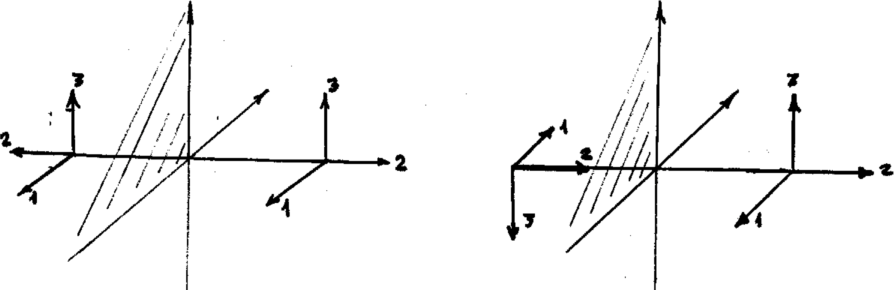
\includegraphics[width=0.6\textwidth]{images/fig_ft1_reflexvect.pdf}	 
	\end{center}
	\caption{}
\end{figure} 

Una reflexión más una rotación permite eliminar componentes de campo.
Una simetría más una rotación-traslación permite eliminar dependencias.

Lo primero que debe hacerse es escribir bien la \vb{J} a partir del dato de la corriente
(que es el que se suele tener) mediante
\[
	i = \int_S \vb{J} \cdot d \vb{S}
\]
En cambio, para \vb{A} es más fácil usar
\[
	\vb{B} = \rotorm{A}
\]
y despejar de aquí la ecuación diferencial que emplear
\[
	\vb{A} = \frac{1}{c} \int_V \frac{\vb{J}}{|\vb{x}-\vb{x}'|} dV
\]


\section{El potencial vector}

Por la ley de Biot y Savart,
\[
	\vb{B} = \frac{1}{c} \int_{V'} \frac{\vb{J}(\vb{x}') \times (\vb{x}-\vb{x}')}{|\vb{x}-\vb{x}'|^3} 
	dV' = \Nabla_x \times \frac{1}{c} \int_{V'} \frac{\vb{J}(\vb{x}')}{|\vb{x}-\vb{x}'|} dV'
\]
de modo que
\be
	\vb{A} = \frac{1}{c} \int_{V'} \frac{\vb{J}(\vb{x}')}{|\vb{x}-\vb{x}'|} dV'
	\label{potvec}
\ee
pero 
\[
	\vb{A}' \equiv \vb{A} + \Nabla \Psi
\]
es tan buen potencial vector como \vb{A} puesto que los rotores verifican $\rotorm{A}=\rotorm{A}'=\vb{B}$,
de lo cual extraemos en conclusión que el potencial vector está definido a menos del gradiente de una
función escalar.

Tomándole el rotor a \eqref{potvec} y considerando $\Nabla'\cdot\vb{J}(\vb{x}')=0$ lo cual se verifica si
la corriente es estacionaria se tiene 
\[
	\rotorm{B} = \frac{4\pi}{c} \vb{J}(\vb{x})
\]
y entonces
\[
	\int_S \rotorm{B} \cdot d\vb{S} = \frac{4\pi}{c} \int_S \vb{J}(\vb{x}) \cdot d\vb{S}
\]
y por el teorema de Stokes arribamos a
\[
	\int_{\Gamma\equiv\partial S} \vb{B}\cdot d\vb{\ell} = \frac{4\pi}{c} I_\Gamma
\]
que es la ley de Ampere. Notemos que $I_\Gamma$ es la corriente concatenada por el lazo $\Gamma$.
Además
\[
	\rotorm{B} = \Nabla\times(\rotorm{A}) = \Nabla(\divem{A}) - \nabla^2 \vb{A} = \frac{4\pi}{c}\vb{J}
\]
pero utilizando el gauge de Coulomb es $\divem{A}=0$ y entonces
\[
	\nabla^2 \vb{A} = -\frac{4\pi}{c}\vb{J}
\]
que es una ecuación de Poisson vectorial.

Magnetostática y electrostáctica son gobernadas por ecuaciones de Poisson para potenciales $\vb{A},\phi$ y
el problema entonces se reduce a resolverlas para luego hallar los campos por derivación.

\section{Unicidad de problemas de potencial}

Si dos problemas satisfacen iguales condiciones de contorno entonces en el recinto encerrado por
ese contorno tienen igual solución.

Si en un recinto $R$
\be
	\phi_1|_{cont} = \phi_2|_{cont}
	\label{potnounico}
\ee
pero se da para el interior de $R$ que $\phi_1\neq\phi_2$ entonces se tiene sucesivamente
\[
	U \equiv \phi_1 - \phi_2 \qquad \qquad \Nabla U = \Nabla \phi_1 - \Nabla \phi_2
\]
\[
	\lapm{U} = \lapm{\phi_1} - \lapm{\phi_2} = -4\pi \rho + 4\pi\rho = 0
\]
\[
	\Nabla\cdot\left( U\Nabla U \right) = U\left( \Nabla\cdot\Nabla U \right) + \Nabla U \cdot \Nabla U
\]
\[
	\int_V \Nabla\cdot\left( U\Nabla U \right) dV = \int_V U \lapm{U}  + (\lapm{U})^2 dV =  \int_V (\lapm{U})^2 dV
\]
llegando al último miembro porque el potencial $U$ cumple la ecuación de Laplace. Luego,
\[
	\int_V (\lapm{U})^2 dV = \int_S U\Nabla{U} \cdot d\vb{S} = 0
\]
habiéndose pasado a la integral de superficie por el teorema de la divergencia y anulando el valor global porque 
$U$ en el contorno es nula (recuérdese \eqref{potnounico}). Además, 
\[
	\Nabla{U} \cdot d\vb{S}  \longrightarrow \left.\dpar{U}{\hat{n}}\right|_{cont}
\]
luego,
\[
	\Nabla U = 0 \qquad \Nabla\phi_1 = \Nabla\phi_2 
\]
y entonces
\[
	\phi_1 = \phi_2 .
\]
a menos, por supuesto, de una constante.



% \bibliographystyle{CBFT-apa-good}	% (uses file "apa-good.bst")
% \bibliography{CBFT.Referencias} % La base de datos bibliográfica

\end{document}
